%---------- Inleiding ---------------------------------------------------------

\section{Introductie}%
\label{sec:introductie}

In een tijd waarin data als het digitale goud beschouwd wordt, groeit de relevantie van webscraping exponentieel.
Webscraping, een techniek gericht op het geautomatiseerd onttrekken van data van websites, komt voort uit de toenemende 
erkenning van data als drijvende kracht achter zakelijke strategieën, wetenschappelijk onderzoek en artificiële intelligentie~\autocite{Oeztuerk2023}.

Bedrijven en organisaties zijn zich steeds meer bewust van de waarde van accurate, actuele data om competitief te blijven
en te anticiperen op veranderende marktomstandigheden. In deze tijd van datagestuurde besluitvorming werkt webscraping als
een krachtige tool om relevevante, real-time data te verkrijgen.

Naast de stijgende behoefte aan gegevens voor zakelijke toepassingen, ondersteunt webscraping ook technologische innovatie. 
De vooruitgang in technologieën zoals artificiële intelligentie, machine learning en big data-analyse vergroot de mogelijkheden
van wat er met de verzamelde gegevens kan worden gedaan.
Traditionele webscrapingmethoden, die zich baseren op het parsen van HTML-code, zijn vaak inefficiënt, inflexibel en gevoelig voor anti-scrapingmaatregelen.
Netwerkverkeersanalyse biedt een innovatieve oplossing voor deze uitdaging. Door het analyseren van het netwerkverkeer dat tussen een browser en een website verloopt, 
kan data in real-time worden geëxtraheerd, zelfs wanneer deze niet expliciet in de HTML-code is gedefinieerd. Dit opent de deur naar een nieuw niveau van efficiëntie en 
flexibiliteit in webscraping.
\\
\\
Deze paper verkent de mogelijkheden van webscraping via netwerkverkeersanalyse, met specifieke focus op het extraheren van JSON-objecten. JSON is een populair formaat voor 
data-uitwisseling en wordt vaak gebruikt om API-responses te serialiseren. JSON (JavaScript Object Notation) is een lichtgewicht, gestandaardiseerd dataformaat.
JSON wordt gebruikt voor het uitwisselen van data tussen verschillende applicaties en programmeertaal vanwege de eenvoud en flexibiliteit die het bied.
Door JSON-objecten te extraheren uit netwerkverkeer kunnen we waardevolle data ontsluiten 
die anders ontoegankelijk zou zijn. Het doel van dit onderzoek is om een antwoord te vinden op de vraag hoe netwerkverkeersanalyse kan worden toegepast voor webscraping,
met specifieke aandacht voor het extraheren van JSON-objecten. Hierbij worden ook volgende deelvragen behandeld:
\begin{itemize}
  \item Welke tools en technieken zijn beschikbaar voor het analyseren van netwerkverkeer voor webscraping?
  \item Hoe kunnen JSON-objecten in netwerkverkeer worden geidentificeerd en gedecodeerd?
  \item Wat zijn de voordelen en nadelen van webscraping via netwerkverkeersanalyse in vergelijking met traditionele methoden?
  \item Welke ethische aspecten zijn er verbonden aan het gebruik van deze methode?
\end{itemize}
Dit is een toegepast onderzoek om de haalbaarheid en prestaties van webscraping via netwerkverkeersanalyse te evalueren. De resultaten worden vergeleken met die van de traditionele
webscraping technieken en formuleren richtlijnen voor verantwoord gebruik van deze methodes. Deze paper belicht ook de ethische aspecten van webscraping via netwerkverkeersanalyse,
met aandacht voor privacy, gegevensbescherming en intellectueel eigendom.

%---------- Stand van zaken ---------------------------------------------------

\section{Literatuurstudie}
\label{sec:Literatuurstudie}
In de digitale wereld van vandaag is data de sleutel tot succes. Bedrijven verzamelen en analyseren data om hun klanten beter te begrijpen, 
hun marketingstrategieën te optimaliseren, en hun concurrentiepositie te versterken. Deze enorme vraag naar kwalitatieve data drijft de ontwikkeling 
van nieuwe en innovatieve methodes voor dataverzameling. Er zijn vele manieren waarop er aan dataverzameling kan gedaan worden, deze studie focussed
zich op webscraping.

\subsection{Webscraping}
\label{sec:Webscraping}
Webscraping is een techniek die automatisch data extraheert van websites. Deze data kan in verschillende formaten
voorkomen, zoals HTML, JSON, XML en CSV. Webscraping heeft tal van toepassingen, waaronder:
\begin{itemize}
  \item Data-extractie is het verzamelen van data van websites voor diverse doeleinden, 
      zoals marktonderzoek,prijsvergelijking en het verzamelen van recensies
  \item Het automatiseren van taken die anders handmatig zouden moeten worden uitgevoerd, denk maar 
  aan het invullen van bepaalde formuliers, aanmaken van documenten en downloaden van bestanden
  \item Monitoren van websites voor veranderingen van prijzen, nieuwe producten of statusen van bepaalde zaken
\end{itemize}

De traditionele webscrapingmethodes baseren zich op het parsen van de HTML-code van webpaginas.
Dit kan gedaan worden met behulp van diverse tools, voornamelijk python libraries, zoals BeautifulSoup, Srapy en Selenium.
In JavaScript heb je dan weer Cheerio en Puppeteer en in Java heb je Jsoup. De voordelen van deze methodes zijn
dat ze eenvoudig zijn aangezien iedere website HTML gebruikt en het dus relatief eenvoudig is om dit te implementeren.
De nadelen van hiervan 

% Voor literatuurverwijzingen zijn er twee belangrijke commando's:
% \autocite{KEY} => (Auteur, jaartal) Gebruik dit als de naam van de auteur
%   geen onderdeel is van de zin.
% \textcite{KEY} => Auteur (jaartal)  Gebruik dit als de auteursnaam wel een
%   functie heeft in de zin (bv. ``Uit onderzoek door Doll & Hill (1954) bleek
%   ...'')


%---------- Methodologie ------------------------------------------------------
\section{Methodologie}%
\label{sec:methodologie}
Het onderzoek is verdeeld in verscheidene fasen om een correcte en grondige evaluatie te kunnen maken van de verschillende talen
en libraries voor het webscrapen. Er wordt bij iedere fase gefocused op een specifiek doel en draagt bij aan het bepalen welke
programmeertaal het meest geschikt is voor webscrapen.

\subsection{Fase 1: Literatuurstudie (3 weken)}
De initiële fase van dit onderzoek richt zich op een grondige literatuurstudie om inzicht te krijgen in bestaande webscraping-tools in Python,
JavaScript en Java. Het onderzoek omvat een gedetailleerde analyse van beschikbare libraries en frameworks, 
waarbij functionaliteiten, gebruiksgemak en efficiëntie worden onderzocht. Deze literaire verkenning legt de 
basis voor het identificeren van geschikte tools voor webscraping in de verdere stadia van het onderzoek.

\subsection{Fase 2: Long list (2 weken)}
Na de literatuurstudie wordt een uitgebreide lijst samengesteld met diverse webscraping-tools voor elke programmeertaal. 
Op basis van de literatuurstudie wordt bepaald welke items op deze long list komen en welke niet. Belangrijke kenmerken van elke tool 
worden zorgvuldig gedocumenteerd. Deze Long List fungeert als een uitgangspunt voor het selectieproces in de volgende fase 
van het onderzoek.

\subsection{Fase 3: Short list (2 weken)}
De selectie van de meest belovende tools vindt plaats in de Short List-fase. De tools op de Long List worden beoordeeld op 
criteria zoals relevantie, gemeenschapsondersteuning en functionaliteit. 
De gekozen tools worden gedocumenteerd als de focus van verdere evaluatie, terwijl minder geschikte opties 
worden uitgesloten.

\subsection{Fase 4: Proof of Concept (5 weken)}
De Proof of Concept fase omvat de ontwikkeling van webscrapers in de geselecteerde tools voor elk van de drie programmeertalen. 
Deze implementatie is gericht op het evalueren van de efficiëntie, schaalbaarheid en praktische toepasbaarheid van elke tool. 
Representatieve webscraping-scenario's worden geïdentificeerd en de ontwikkelde PoC's worden onderworpen aan metingen van 
uitvoeringstijd, geheugengebruik en schaalbaarheid. De codecomplexiteit en praktische bruikbaarheid van elke tool worden 
nauwkeurig beoordeeld.

\subsection{Conclusie (1 week)}
De afsluitende fase van het onderzoek omvat de analyse van bevindingen uit zowel de literatuurstudie als de PoC-fase. 
Resultaten van de vergelijkende metingen tussen programmeertalen worden geëvalueerd, en conclusies worden geformuleerd over de 
geschiktheid van Python, JavaScript en Java voor webscraping-taken.
%---------- Verwachte resultaten ----------------------------------------------
\section{Verwacht resultaat, conclusie}%
\label{sec:verwachte_resultaten}
De verwachte resultaten van dit onderzoek worden gedefinieerd door meetbare uitkomsten voortkomend uit zowel de literatuurstudie 
als de Proof of Concept (PoC)-fase. Deze resultaten zullen concreet worden weergegeven in vergelijkende grafieken, waarbij de 
programmeertalen Python, JavaScript en Java worden geëvalueerd op basis van verschillende webscraping-scenario's. 
De assen van deze grafieken vertegenwoordigen de programmeertalen (x-as) en metingen zoals uitvoeringstijd en geheugengebruik. (y-as)
\\
\\
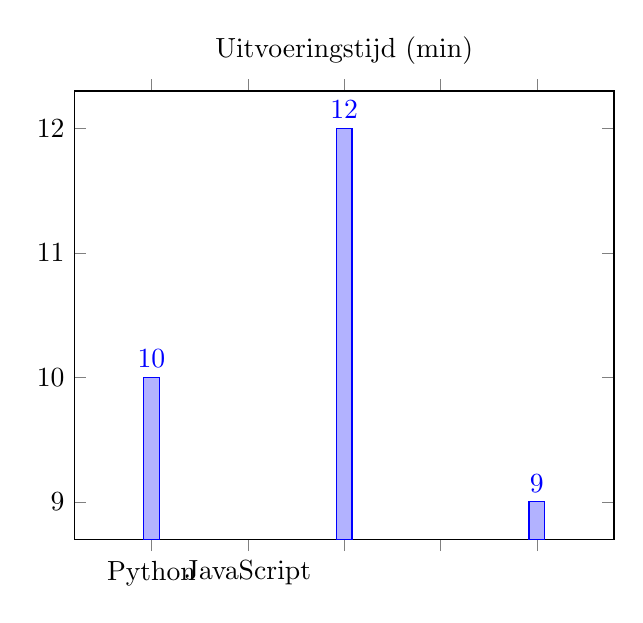
\begin{tikzpicture}
\begin{axis}[
  title=Uitvoeringstijd (min),
  ybar,
  nodes near coords,
  bar width=0.2cm,
  symbolic x coords={Java,Python,Javascript},
  enlarge x limits=.2,
  xticklabels={Java,Python,JavaScript},
]

\addplot coordinates {
  (Java,10)
  (Python,12)
  (Javascript,9)
};

\end{axis}
\end{tikzpicture}
  
Een aanvullend aspect van de verwachte resultaten omvat de beoordeling van codecomplexiteit en praktische bruikbaarheid in webscraping
-implementaties voor elke taal.

De meerwaarde van dit onderzoek voor de doelgroep ligt in de mogelijkheid om optimalere technologische keuzes te maken. 
Door inzicht te verschaffen in de prestaties van Python, JavaScript en Java, biedt dit onderzoek een waardevolle leidraad. 